\documentclass[12pt,twoside]{article}
\usepackage{jmlda}
\usepackage[utf8]{inputenc}
\usepackage[russian]{babel}
\usepackage[T2A]{fontenc}
\usepackage{lineno}
\usepackage{graphicx}
\graphicspath{{pictures/}}
\DeclareGraphicsExtensions{.pdf,.png,.jpg}
\linenumbers
\usepackage{setspace}
\doublespacing


\usepackage[left=1.5cm,right=1.5cm,
    top=2cm,bottom=2cm,bindingoffset=0cm]{geometry}

\newcommand{\norm}[1]{\left\lVert#1\right\rVert}

\title
    [Построение оптимальной системы нейрокомпьютерного интерфейса]
    {Прогнозирование намерений. Построение оптимальной модели декодирования сигналов при моделировании нейрокомпьютерного интерфейса.}
\author {Кудрявцева П.Ю.} % основной список авторов, выводимый в оглавление
\email{polinakud13@gmail.com}
\thanks
    {Научный руководитель:  Стрижов~В.\,В.
    Консультант:  Исаченко~Р.\,В.}
\organization
    {$^1$Московский физико-технический институт (МФТИ)}
\abstract
    {При построении систем нейрокомпьютерного интерфейса возникает проблема наличия зависимости в исходных данных. Для построения устойчивой прогностической модели необходимо провести процедуру выбора признаков и снизить размерность исходных данных. В работе предлагается систематический подход к построению модели, учитывающий зависимости в исходном пространстве сигналов и в пространстве целевой переменной. Исследуются алгоритмы построения систем нейрокомпьютерного интерфейса, проведен подробный анализ ошибки различных алгоритмов на реальных данных. Исследовано влияние тензорной структуры данных на качество модели.

\bigskip
\textbf{Ключевые слова}: \emph {отбор признаков, нейрокомпьютерный интерфейс, PLS, QPFS}.}

\begin{document}
\maketitle



\section{Введение}
 Цель работы ~-- построить систему нейрокомпьютерного интерфейса (НКИ). Предлагается декодировать сигналы мозга ECoG/EEG и спрогнозировать движение конечности субъекта. Главной проблемой  является наличие сильной корреляции исходных сигналов. Модель, обученная на избыточных данных, является нестабильной. Необходимо избавиться от лишних зависимостей. Для этого применяются методы снижения размерности пространства и выбора признаков.
 
 В качестве алгоритма снижения размерности в работе используется метод частичных наименьших квадратов \cite{pls_effective}. Этот метод позволяет получить эффективные и информативные линейные комбинации старых признаков. Алгоритм проецирует признаковую матрицу  \textbf{X}  и целевую матрицу  \textbf{Y}  в пространство меньшей размерности, сохраняя максимальное количество информации об исходных матрицах. В новом пространстве признаки в проекции матрицы \textbf{X} линейно независимы. Также, максимизируется взаимосвязь между проекциями. После проецирования максимизируется линейная зависимость между столбцами проекций \cite{pls_ni}. В \cite{elisey} доказана эффективность рекурсивного PLS для быстрой реакции системы НКИ на поступающие сигналы. В \cite{elisey2}, \cite{elisey3}  предложены многомодальные модификации алгоритма PLS. 
 
 Выбор признаков осуществляется алгоритмом выбора признаков с помощью квадратичного программирования (QPFS). Алгоритм формулирует задачу отбора признаков в виде задачи квадратичного программирования. Решение этой задачи позволяет выбрать независимые признаки, релевантные целевому вектору \cite{qpfc}. В \cite{motrenko} исследуется задача выбора признаков для построения систем нейрокомпьютерных интерфейсов. В статье представлена модификация алгоритма QPFS, которая позволяет применять его к многомерным данным, в том числе для задачи построения НКИ. Доказана эффективность модификации алгоритма для большого количества признаков, по сравнению с другими алгоритмами снижения размерности.
 
 В этой статье объединены существующие подходы к решению задачи построения системы НКИ. Предлагается стандарт для декодирования сигналов ECoG/EEG. Предложен алгоритм анализа имеющихся зависимостей в исходных данных. 

\section{Постановка задачи}

Данные ECoG состоят из многомерных временных рядов, содержащих информацию о напряжении на 32 электродах. Задача заключается в предсказании по сигналам ECoG позиции руки субъекта в следующие моменты времени. По данным строится матрица 
признаков $\textbf{X}^\prime \in \mathbb{R}^{m\times h \times 32}$ с $m$ наблюдениями, содержащими $h$ значений напряжения для каждого из 32 электродов, и целевых значений $\textbf{Y}^\prime \in \mathbb{R}^{m\times k}$, где $k$ ~-- координаты позиции руки.

В считываемых данных присутствуют линейные зависимости. Вследствие зависимостей линейная модель, построенная по этим данным, является неустойчивой. Для решения этой проблемы необходимо учитывать корреляцию данных на этапе построения модели и использовать алгоритмы,
снижения размерности, для получения новой матрицы признаков и целевой матрицы.  Для этого проводится снижение размерности данных с использованием алгоритма PLS и выбор признаков с использованием алгоритма QPFS. Алгоритм PLS позволяет получить информативные линейные комбинации исходных признаков в качестве новых признаков, а алгоритм QPFS проводит отбор независимых признаков. Введем обозначения для матриц после применения одного из алгоритмов. Обозначим новую целевую матрицу $X$, где $g(\textbf{X}^\prime) = \textbf{X}$ , $g: \mathbb{R}^{m\times h \times 32} \to \mathbb{R}^{m\times n} $, $n$ - новая размерность матрицы признаков. Новая признаковая матрица $Y$, где $g^\prime(\textbf{Y}^\prime) = \textbf{Y}$, где $g^\prime: \mathbb{R}^{m\times k} \to \mathbb{R}^{m\times r} $, $r$ - новая размерность целевой матрицы. После выделения оптимального признакового пространства предполагается, что между новой матрицей признаков \textbf{X} и \textbf{Y} существует зависимость: $$ \textbf{Y} = f(\boldsymbol{X},\boldsymbol{\Theta}) + \epsilon ,$$ где $\epsilon \in \mathbb{R}^{m\times r}$ ~-- матрица остатков, $ \boldsymbol{\Theta} \in \mathbb{R}^{r\times n}$ ~-- параметры модели. 

Задача прогнозирования положения конечности сводится к поиску матрицы параметров $ \boldsymbol{\Theta}$ по данным \textbf{X}, \textbf{Y}. Оптимальные параметры определяются минимизацией квадратичной функции ошибки:
$$ L( \boldsymbol{\Theta}, \textbf{X}, \textbf{Y}) = \norm{ f(\boldsymbol{X},\boldsymbol{\Theta})  - \textbf{Y}}^2_2 \to \min_{\boldsymbol{\Theta}}. $$ В частности, будет решаться задача при $f(\boldsymbol{X},\boldsymbol{\Theta}) = \boldsymbol{\Theta} \textbf{X}$

\section{Базовый алгоритм}

Используются два алгоритма, PLS и QPFS. 
Алгоритм PLS проецирует исходные матрицы $\textbf{X}^\prime$ и $\textbf{Y}^\prime$ в пространство меньшей размерности, $$\textbf{X} = \textbf{TP}^T + \textbf{F}, \textbf{Y} = \textbf{UQ}^T + \textbf{E} ,$$ где $\textbf{T}, \textbf{U} \in \mathbb{R}^{m \times n}$ 
- образы $\textbf{X}, \textbf{Y}$ в скрытом пространстве, 
$\textbf{P} \in \mathbb{R}^{n \times h \times 32}, \textbf{Q} \in \mathbb{R}^{n \times k}$ - матрицы перехода, 
$\textbf{F} \in \mathbb{R}^{m \times h \times 32}, \textbf{E} \in \mathbb{R}^{m \times k}$ - матрицы остатков. Cтолбцы матрицы $\textbf{T}$ ортогональны. При проецировании максимизируется взаимосвязь между матрицами $\textbf{T, U}$. Алгоритм проводит $n$ шагов, на $k$-ом шаге вычисляются очередные столбцы $\textbf{t}_k,\textbf{u}_k,\textbf{p}_k,\textbf{q}_k$ матриц $\textbf{T, U, P, Q}.$
После нахождения проекций, алгоритм максимизирует линейную зависимость между столбцами матриц $\textbf{T, U}.$

Алгоритм QPFS ставит задачу отбора признаков в виде задачи квадратичного программирования $$\min_x \frac1{2} x^T \textbf{Q}x- \textbf{F}^Tx ,$$
где $x \in \mathbb{R}^l$, $\textbf{Q} \in \mathbb{R}^{l \times l}$ - симметричная положительно определенная матрица, $\textbf{F} \in \mathbb{R}^l$ - вектор с положительными значениями и $l$ - количество признаков в исходной признаковой матрице. Элементы $q_{i,j}$ матрицы $\textbf{Q}$ определяются, как взаимная информация $i$ и $j$ признака. Таким образом, матрица $\textbf{Q}$ является мерой подобия признаков. Элементы $f_i$ вектора $\textbf{F}$ определяются при помощи взаимной информации $i$-го признака и целевой переменной. Вектор $\textbf{F}$ измеряет релевантность каждого признака по отношению к целевой переменной. Задача решается в условиях $x_i \geq 0, i = 1, \dots, l$ и $\sum\limits^l_{i=1} x_i = 1$. Компоненты $x_i$ решения задачи представляют собой веса $i$-го признака. Отбор признаков проводится в зависимости от их веса в векторе решения $x$, выбираются признаки с наибольшими весами.

\section{Эксперимент}





Частоты сигналов с датчиков и соответсвующие им трехмерные координаты кисти в пространстве были разбиты на обучающую и тестовую выборку. Данные были нормализованы так, чтобы среднее каждого признака на обучающей выборке было равно 0, а среднее квадартичное отклонение было равно 1. 

\begin{figure}[h]
\begin{minipage}[h]{0.49\linewidth}
\center{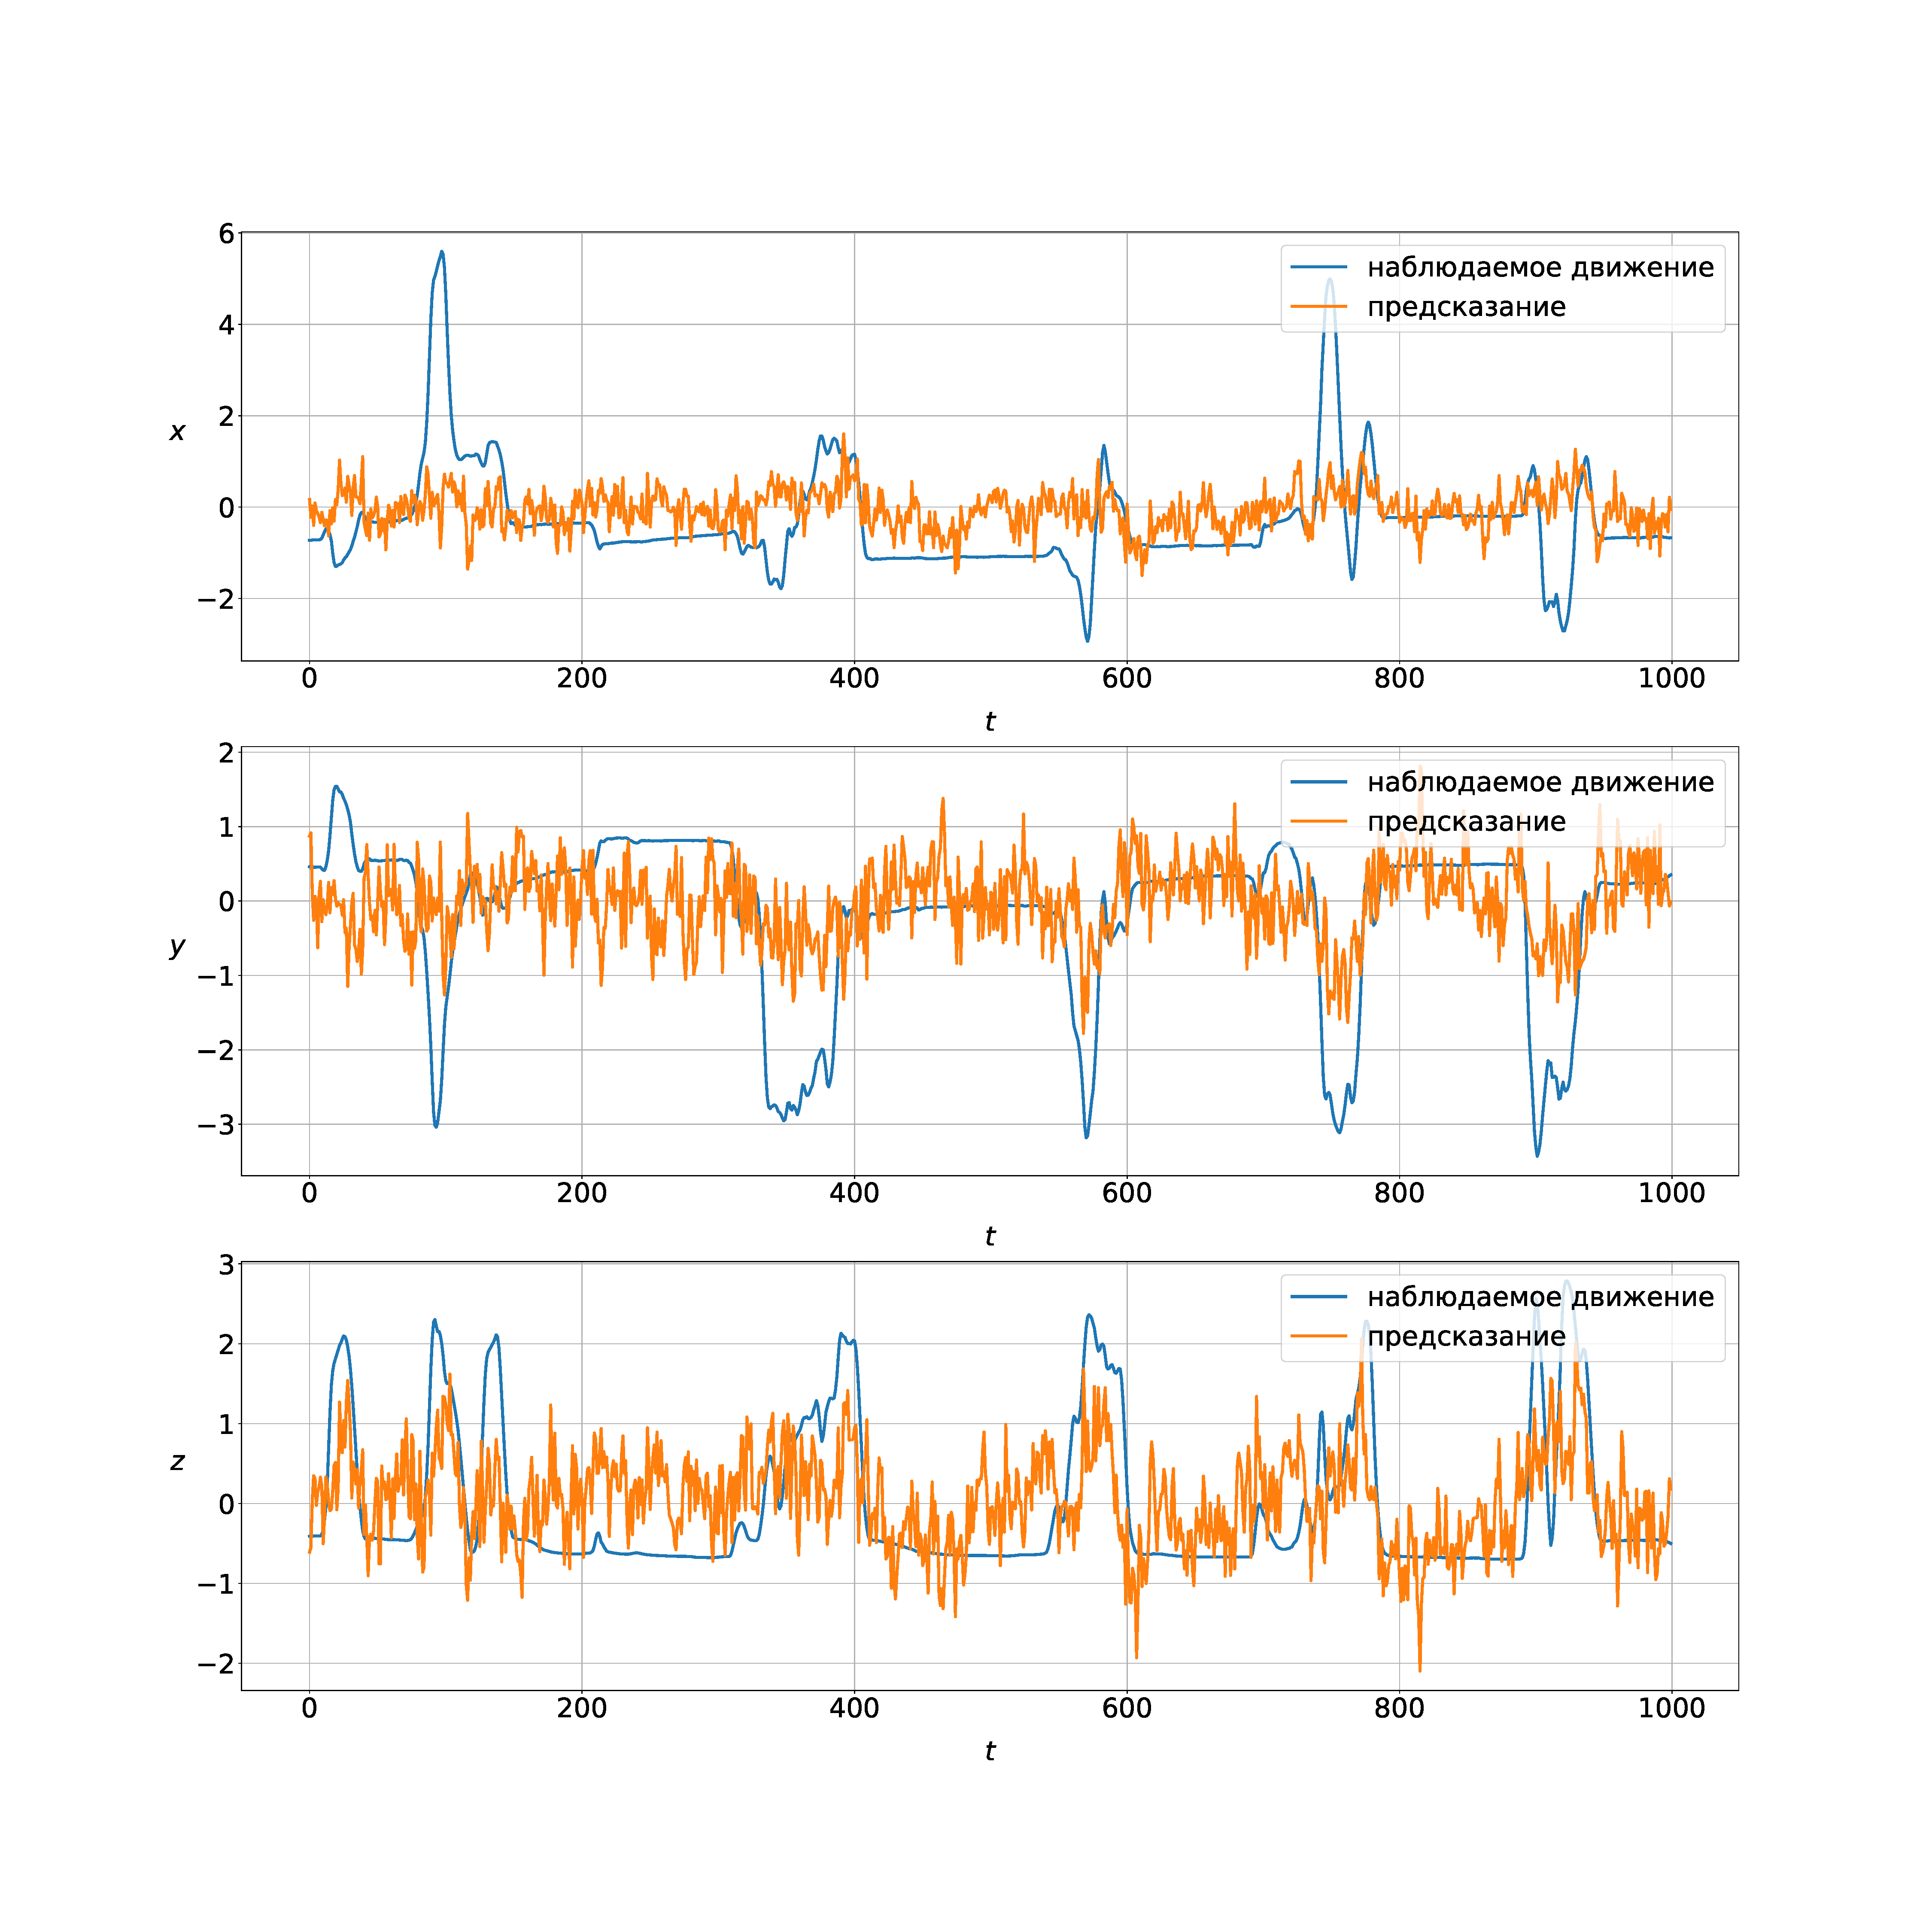
\includegraphics[scale=0.13]{pls_results}}
\caption{Предсказания с помощью алгоритма PLS}
\label{fig:pls_basic}
\end{minipage}
\hfill
\begin{minipage}[h]{0.49\linewidth}
\center{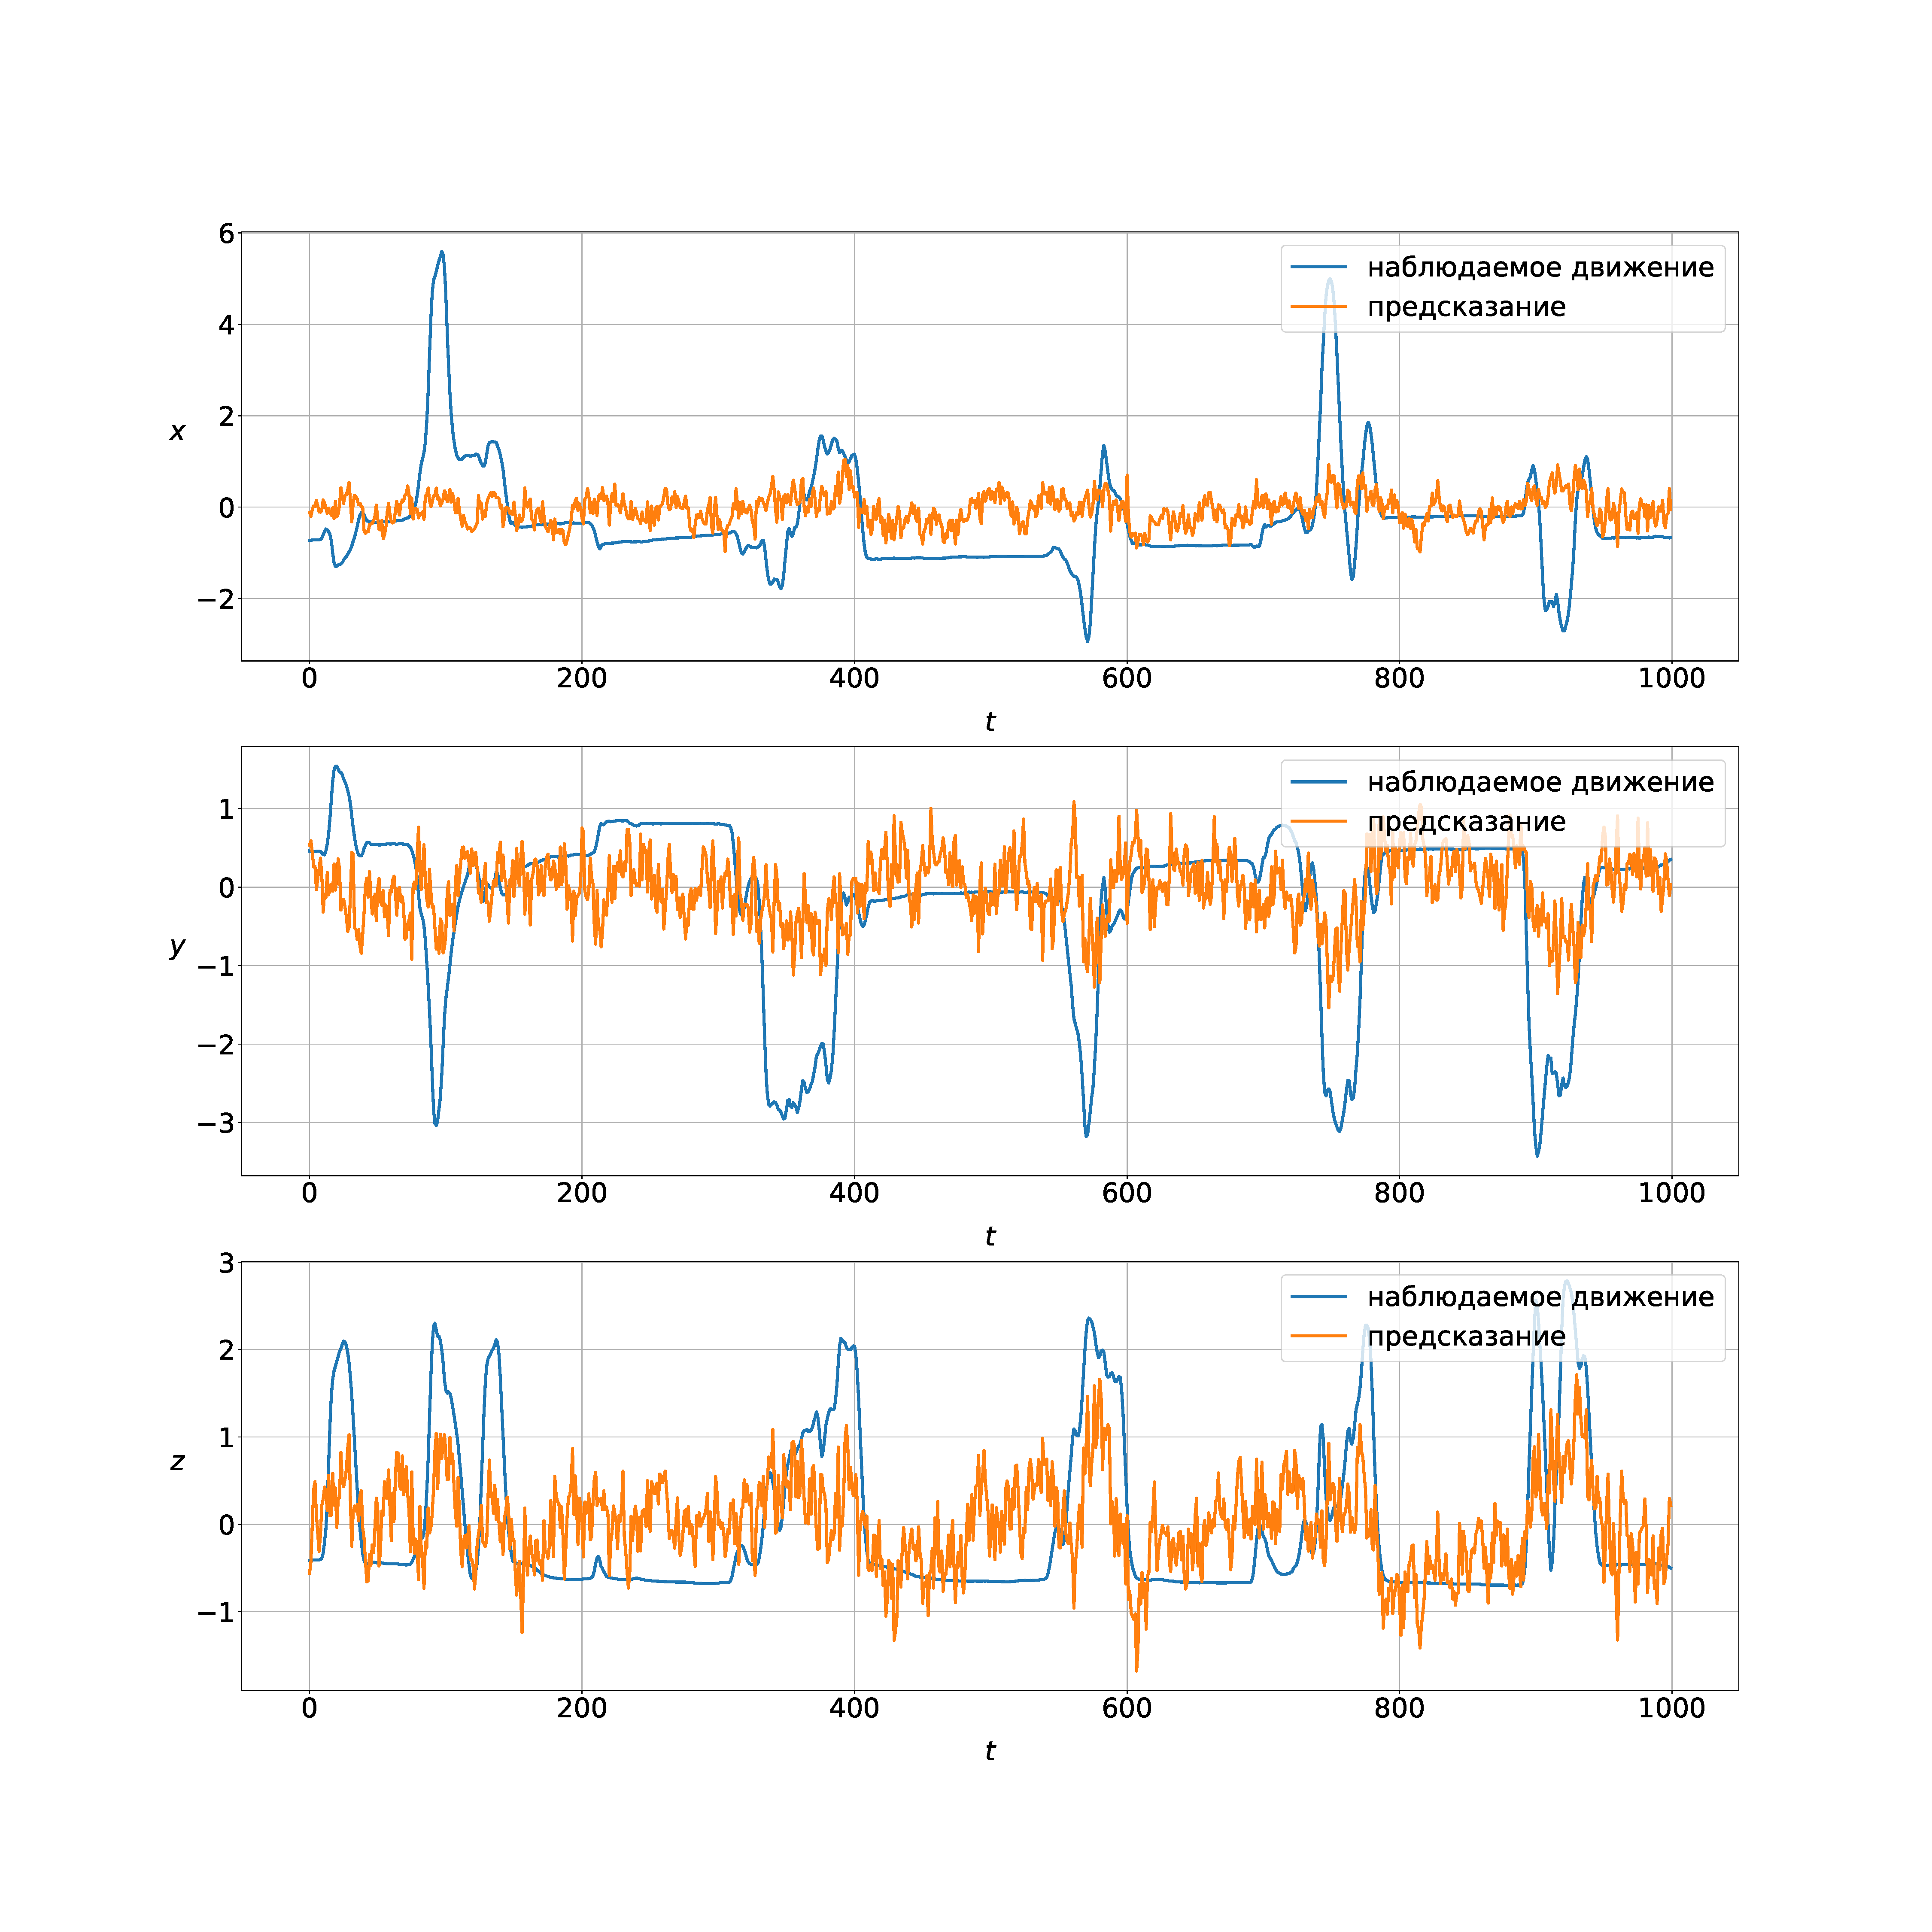
\includegraphics[scale=0.13]{qpfs_results}}
\caption{Предсказания с помощью алгоритма QPFS}
\label{fig:qpfs_basic}
\end{minipage}
\end{figure}


Сначала был запущен алгоритм PLS на обучающей выборке. Путем нескольких запусков алгоритма PLS с различным количеством компонент на обучающей выборке и анализа полученной квадратичной функции ошибки, было выбрано количество компонент, равное 100, для итогового запсука. Значение средней квадратичной функции ошибки на тестово выборке равно 0.945. На графике рис. \ref{fig:pls_basic} представлена зависимость координаты в пространстве от времени. График предсказаний с помощью алгоритма PLS сильно осциллирует. При этом, особенно на последнем графике (для координаты $z$), общий рисунок повторен довольно точно - почти все пики на графике наблюдаемого движения предсказаны корректно. Предсказание координаты $x$, напротив, осциллирует возле константы, совершенно не повторяя рисунок истинной координаты. 

Также на обучающей выборке был запущен алгоритм QPFS. Аналогично PLS, было выбрано оптимальное количество выбранных признаков, равное 100. На этих признаках был запущен алгоритм линейной регрессии. Средняя квадратичная функция ошибки на тестовой выборке равна 0.916, что меньше, чем у алгоритма PLS. На рис. \ref{fig:qpfs_basic} видно, что предсказания алгоритма также осциллируют, но не так сильно, как предсказания PLS. Общий рисунок (пики и падения координат), аналогично PLS, хорошо предсказывается для координаты $z$, и плохо (график осциллирует возле константы), для координаты $x$. 

Оба алгоритма неудовлетворительно справляются с поставленной задачей, но где-то улавливают общую картину.



\bibliography{Kudryavtseva2019Project18}{}
\bibliographystyle{plain}
\end{document}
